%  !TeX  root  =  user_guide.tex

\section{Приступая к работе}\label{label_getstarted}

% when the revision of a section has been finalized,
% comment out the following line:
% \updatedisclaimer

В этой главе дается краткий обзор процесса установки \qg, приводятся
некоторые примеры данных с веб-страницы \qg и показывается пример
рабочего цикла отображения растровых и векторных слоев.

\section{Установка}\label{label_installation}
\index{installation}

Процесс установки \qg очень прост. Пакеты для стандартной установки
доступны для MS Windows и Mac OS X. Для разнообразных дистрибутивов
GNU/Linux предоставляются бинарные пакеты (rpm и deb), или же можно
добавить репозитории программного обеспечения в менеджер программ. Самую
актуальную информацию по бинарным пакетам можно получить на веб-сайте
\qg \url{http://qgis.osgeo.org/download/}.

\minisec{Установка из исходных пакетов}

Если вы хотите собрать \qg из исходных пакетов, обратитесь к Руководству
по программированию и компиляции, доступном на странице
\url{http://qgis.osgeo.org/documentation/}. Инструкции по установке
также распространяются вместе с исходным кодом \qg.

\section{Примеры данных}\label{label_sampledata}
\index{data!sample}

Руководство пользователя содержит шаблоны, основанные на примерах данных
\qg.

\win Установщик для Windows содержит опцию, которая позволяет загрузить
примеры данных \qg. Если опция активна, данные будут загружены в папку
с названием \filename{GIS DataBase} внутри папки \filename{Мои документы}
текущего пользователя. В дальнейшем, можно переместить эту папку в более
удобное место. Если во время первичной установки \qg флажок для загрузки
примеров данных не был отмечен, можно поступить следующим образом:
\begin{itemize}[label=--]
\item использовать имеющиеся данные;
\item загрузить примеры данных с веб-сайта \qg по адресу
\url{http://qgis.osgeo.org/download}; или
\item удалить \qg и переустановить его с выбраной опцией загрузки
примеров данных, только если вышеописанные решение не дадут результата.
\end{itemize}

\nix \osx Для GNU/Linux и Mac OSX пока еще нет установочных пакетов
примеров данных, доступных в виде rpm, deb или dmg. Для использования
примеров данных, необходимо загрузить файл \filename{\qg\_sample\_data}
в виде архива ZIP или TAR по адресу
\url{http://download.osgeo.org/qgis/data/} и распаковать его. Набор
данных Alaska содержит все данные, которые используются как примеры и
снимки экрана в руководстве пользователя, а также содержит небольшую
базу данных GRASS. В примере данных используется проекция Alaska Albers
Equal Area с единицами измерения в футах. Код EPSG (European Petroleum
Survey Group) данной проекции"--- 2964.

\begin{verbatim}
PROJCS["Albers Equal Area",
    GEOGCS["NAD27",
        DATUM["North_American_Datum_1927",
            SPHEROID["Clarke 1866",6378206.4,294.978698213898,
                AUTHORITY["EPSG","7008"]],
            TOWGS84[-3,142,183,0,0,0,0],
            AUTHORITY["EPSG","6267"]],
        PRIMEM["Greenwich",0,
            AUTHORITY["EPSG","8901"]],
        UNIT["degree",0.0174532925199433,
            AUTHORITY["EPSG","9108"]],
        AUTHORITY["EPSG","4267"]],
    PROJECTION["Albers_Conic_Equal_Area"],
    PARAMETER["standard_parallel_1",55],
    PARAMETER["standard_parallel_2",65],
    PARAMETER["latitude_of_center",50],
    PARAMETER["longitude_of_center",-154],
    PARAMETER["false_easting",0],
    PARAMETER["false_northing",0],
    UNIT["us_survey_feet",0.3048006096012192]]
\end{verbatim}

Если вы собираетесь использовать \qg как графический интерфейс для
GRASS, на официальном веб-сайте ГИС GRASS \\
\url{http://grass.osgeo.org/download/data.php} можно найти примеры
областей (например Spearfish или South Dakota).

\section{Пример рабочего цикла}\label{samplesession}

Теперь, когда \qg установлен и доступны примеры данных, мы хотим
показать короткий и простой пример рабочего цикла \qg. Будем
визуализировать растровый и векторный слои, используя
почвенно-растительный покров как слой растра
\filename{\qg\_sample\_data/raster/landcover.img} и озера как векторный
слой \filename{\qg\_sample\_data/gml/lakes.gml}.

\minisec{Запуск \qg}

\begin{itemize}[label=--]
\item \nix{Запустите \qg набрав: \usertext{\qg} в командной строке, или
используйте меню Приложения, если используются предварительно
скомпилированные бинарные файлы.}
\item \win{Запустите \qg используя меню Пуск или ярлык на Рабочем Столе,
или двойным нажатием на файле проекта \qg.}
\item \osx{Дважды нажмите на значке в папке Приложения.}
\end{itemize}

\begin{figure}[ht]
   \centering
   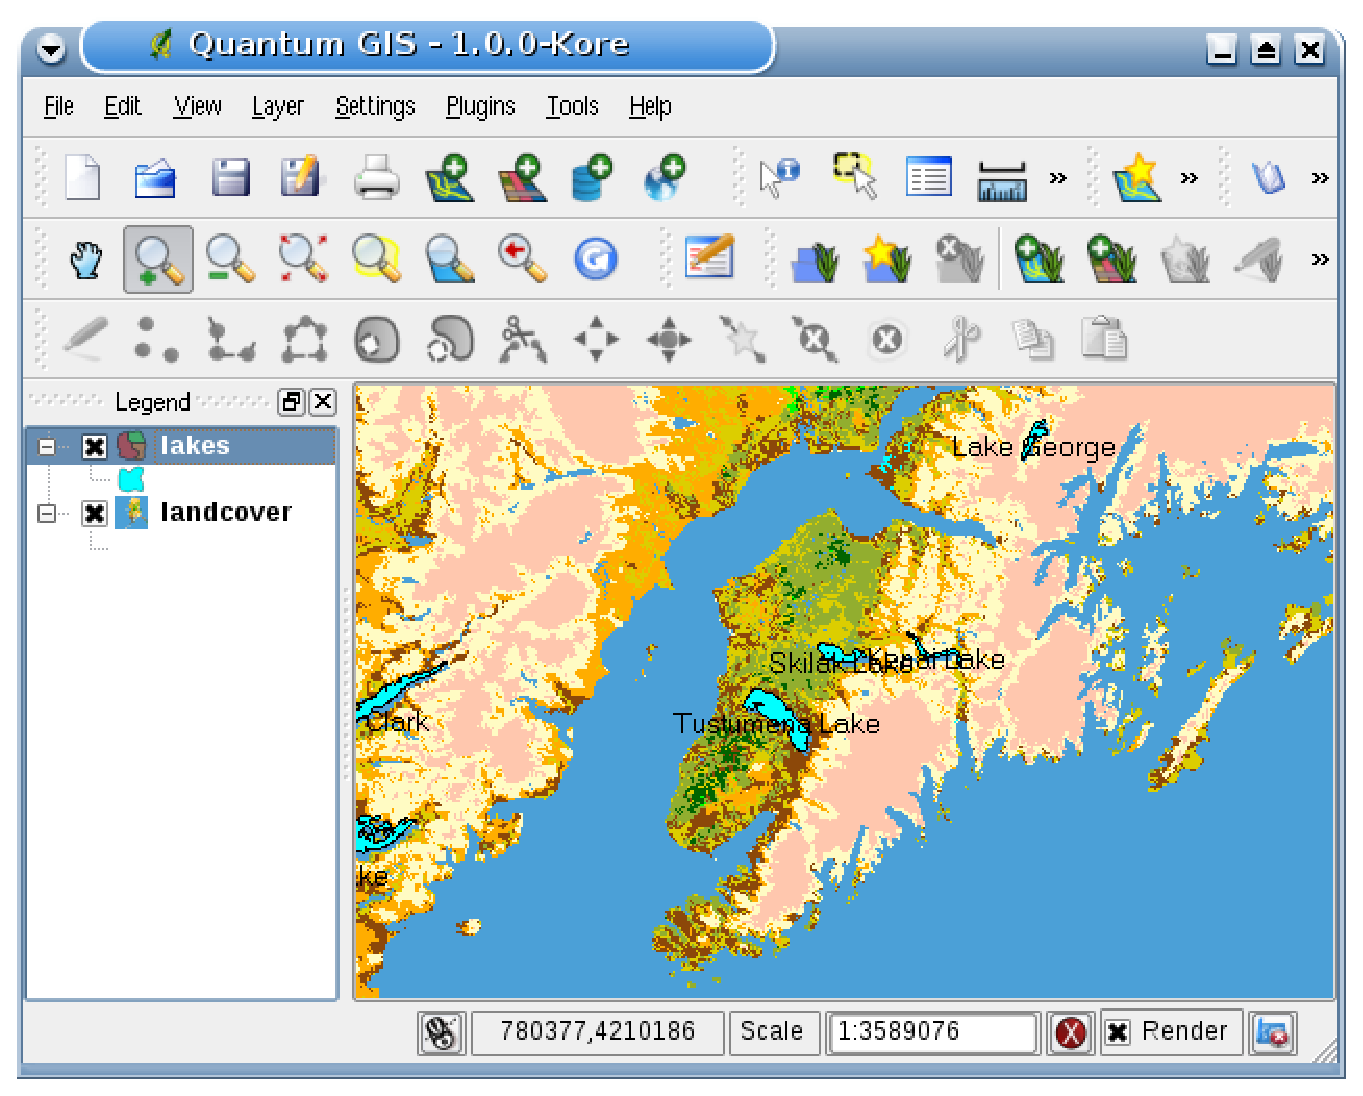
\includegraphics[clip=true, width=12cm]{simple_session}
   \caption{Пример рабочего цикла \qg \nixcaption}\label{fig:simple_session}
\end{figure}

\minisec{Загрузка слоев растра и вектора из примеров данных}

{\setlength{\baselineskip}{1.3\baselineskip}
\begin{enumerate}[itemsep=2pt]
\item Нажмите на значке \toolbtntwo{mActionAddRasterLayer}{Добавить растровый слой}.
\item Откройте папку \filename{\qg\_sample\_data/raster/}, выберите файл
формата ERDAS Img \filename{landcover.img} и нажмите \button{Открыть}.
\item Если нужного файла нет в списке, проверьте, правильно ли указан
тип файлов в нижней части диалогового окна, в данном случае
<<Erdas Imagine Images (*.img, *.IMG)>>
\item Теперь нажмите на значке \toolbtntwo{mActionAddOgrLayer}{Добавить векторный слой}.
\item \radiobuttonon{'Файл'} должен быть выбран как Тип источника в
новом окне \dialog{Добавить векторный слой}. Теперь нажмите \button{Обзор},
чтобы выбрать векторный слой.
\item Откройте папку \filename{\qg\_sample\_data/gml/}, выберите <<GML>>
в выпадающем списке Тип файлов, затем выберите файл GML (Geography Markup
Language) \filename{lakes.gml} и нажмите \button{Открыть}, затем в окне
Добавить векторный слой нажмите \button{Открыть}.
\item Немного увеличьте изображение территории с озерами.
\item Дважды нажмите на слое \filename{lakes} в окне Слои, чтобы открыть
окно \dialog{Свойства слоя}.
\item Нажмите на вкладке \tab{Символика} и выберите синий в качестве
цвета заливки.
\item Нажмите на вкладке \tab{Подписи} и включите флажок
\checkbox{Включить подписи} для отображения подписей. Выберите значение
NAMES в Поле, содержащее подпись.
\item Для улучшения читаемости подписей, можно добавить буфер белого
цвета вокруг них, включив флажок \checkbox{Буферизовать подписи} и
выбрав Размер буфера 3.
\item Нажмите \button{Применить}, проверьте, устраивает ли результат и,
наконец, нажмите \button{ОК}.
\end{enumerate}
\par}
Видите, как просто отобразить растровые и векторные слои в \qg. Продолжим,
перейдя к разделам, которые больше расскажут о доступной функциональности,
возможностях и настройках, и как это использовать.

\FloatBarrier
